%% Los cap'itulos inician con \chapter{T'itulo}, estos aparecen numerados y
%% se incluyen en el 'indice general.
%%
%% Recuerda que aqu'i ya puedes escribir acentos como: 'a, 'e, 'i, etc.
%% La letra n con tilde es: 'n.



\chapter{Métodos}
%\setcounter{section}{1}
\section{Paquete de R}

%https://oscarperpinan.github.io/R/Paquetes.html 
Una librería o paquete (\emph{package}) es una colección de objetos creados y organizados siguiendo un protocolo fijo que garantiza un soporte mínimo para el usuario así como la ausencia de errores (de sintaxis) en la programación.

\section{Creación del paquete de R}
Los pasos necesarios para la creación de un paquete son:
\begin{itemize}
\item Creación de los objetos que contendrá el paquete (funciones y/o
datos).
\item Creación del esqueleto del paquete.
\item Redacción de la documentación.
\item Compilación del paquete en Linux y creación de la versión para Windows.
\item Instalación.
\item Prueba y publicación.
\end{itemize}

\subsection{Objetos del paquete}
Un paquete puede contener cualquier tipo de objetos de R : funciones, datos etc. Lo primero que debe hacerse es programar las funciones y preparar los datos. El proceso de creación vigila que no hayan errores sintácticos pero no controla si hay errores lógicos.
 
\subsection{Esqueleto y estructura del paquete}
R proporciona una función \emph{package.skeleton} que permite automatizar el proceso de creación de un paquete creando los directorios, los archivos de documentación y otros objetos necesarios.
La  siguiente instrucción construye la estructura de un paquete llamado \emph{geneticae}, 

\begin{lstlisting}[frame=single]
package.skeleton(name = geneticae)
\end{lstlisting}

creando una carpeta de nombre \emph{geneticae} con 3 sub-carpetas en el directorio de trabajo y tres archivos sin extensión. Estos ultimos son los siguintes: 
\begin{itemize}

\item DESCRIPTION: contenido básico para
documentar según la descripción del paquete:

Package: geneticae\\
Type: Package\\
Title: What the package does (short line)\\
Version: 1.0\\
Date: 2019-09-21\\
Author: Who wrote it\\
Maintainer: Who to complain to <yourfault@somewhere.net>\\
Description: More about what it does (maybe more than one line)\\
License: What license is it under?\\

\item NAMESPACE: R usa un sistema de gestión de espacio de nombres que permite al autor del paquete especificar:
\begin{itemize}
\item las variables del paquete que se exportan (y son, por tanto, accesibles a los usuarios)
\item las variables que se importan de otros paquetes.
\item las clases y métodos S3 y S4 que deben registrarse.
\end{itemize}

Este mecanismo queda definido en el contenido del fichero NAMESPACE.

\item Read-and-delete-me: contiene algunas instrucciones importantes sobre cómo personalizar el paquete.
\end{itemize}

Las siguientes son las 3 sub-carpetas creadas:

\begin{itemize}
\item La carpeta \textbf{data} contiene todos los archivos correspondientes a los datos comprimidos con el nombre con el que fueron creados, con la extensión .rda. Estos no pueden ser modificados.
\item La carpeta \textbf{man} contiene todos los archivos de extensión .Rd y un archivo por objeto creado (datos o programa). Estos documentos son parte del sistema de ayuda del paquete en PDF y en HTML; por este motivo, la escritura sigue las reglas de LaTeX.
\item La carpeta \textbf{R} contiene todos los programas fuente, siendo .R la extensión de los mismos.
\end{itemize}
La documentación es uno de los aspectos mas importantes del código, sin ella, los usuarios no sabrán cómo usar el paquete. R proporciona una forma estándar de documentar paquetes: escribir archivos .Rd en la carpeta man, los cuales utilizan una sintaxis personalizada, basada en LaTeX. Sin embargo, el paquete \emph{roxygen2}, utilizado en este trabajo, permite obtener la documentación de una manera sencilla, proporcionando una serie de ventajas sobre la escritura los archivos .Rd:

\begin{itemize}
\item El código y la documentación son adyacentes, de modo que cuando el código se modifique, será fácil actualizar la documentación.

\item Inspecciona dinámicamente los objetos que está documentando, para que pueda agregar automáticamente los datos que de otra forma se deben escribir a mano.

\item Resume las diferencias en la documentación de los métodos S3 y S4, los genéricos y las clases, por lo que necesita aprender menos detalles.
\end{itemize}

Además de generar archivos .Rd, \emph{roxygen2} también creará un archivo NAMESPACE y administrará el campo \emph{Imports} del archivo DESCRIPTION.


\subsection{Compilación e instalación}
Una vez creada la documentación se debe chequear el paquete y generar los instaladores con su corresponiente manual. Para ello se utilizan las siguiente funciones:
\begin{itemize}
\item \emph{R CMD check} verificará que no haya errores de sintaxis o no se generen warnings. Está compuesto por más de 50 chequeos individuales entre los cuales se encuentran: la estructura del paquete, el archivo descripción, namespace, el código de R, los datos, la documentación, entre otros.
\item  \emph{R CMD build} compilará el paquete generando un archivo geneticae.tar.gz listo para su instalación en Linux y \emph{RCMD build -binary} generará el archivo para la instalación en Windows.
\item \emph{RCMD Rd2dvi --pdf} preparará el manual y \emph{R CMD INSTALL} instalará el paquete dejándolo listo para su uso
\end{itemize}

\subsection{Publicación}
%https://rsanchezs.gitbooks.io/ciencia-de-datos-con-r/paquetes/paquetes.html
Un repositorio es el lugar dónde están alojados los paquetes y desde el cuál se pueden descargarlos. Entre los repositorios más populares de paquetes R se encuentran:

\begin{itemize}
\item \textbf{CRAN}: es el principal repositorio de paquetes de R, está coordinado por la fundación R. Previa a la publicación en este repositorio el paquete debe pasar por diferentes pruebas para asegurar que cumple con las políticas de CRAN.

\item \textbf{Bioconductor}: se trata de un repositorio específico para bioinformática. Del mismo modo que CRAN, tiene sus propias políticas de publicaciones y procesos de revisión.

\item \textbf{GitHub}: a pesar que no es específico para R, github es con toda seguridad el repositorio más popular para la publicación de proyectos \emph{open source} (del inglés, código abierto). Su popularidad procede del espacio ilimitado que proporciona para el alojamiento de proyectos \emph{open source}, la integración con git (un software de control de versiones) y, la facilidad de compartir y colaborar con otras personas. Una de sus desventajas es que no proporciona procesos de control.

\item \textbf{R-Forge} y \textbf{RForge}: son entornos de desarrollo de paquetes y repositorios. Eso significa que incluyen control de fuente, seguimiento de errores y otras características. Puede obtener versiones de desarrollo de paquetes de estos.
\end{itemize}

El paquete \emph{geneticae} se encuentra en GitHub, para instalar el mismo (o cualquiera que se encuentre en dicho repositorio) se deben seguir las siguientes instrucciones:\\


\begin{lstlisting}[frame=single]
install.packages(remotes) 
library(remotes)
install_github(jangelini/geneticae) 
\end{lstlisting}


{\Huge{FALTAN LAS COMILLITAS EN INSTALL Y EN EL USUARIO DE GITHUB.. ME DA ERROR CUANDO LAS PONGO}}



{\Huge{(Ideas de: TRABAJO FINAL P SHINY)}}

\section{Aplicación Web}
Una aplicación web es una aplicación o herramienta informática accesible desde cualquier navegador, bien sea a través de internet (lo habitual) o bien a través de una red local. 
Estas aplicaciones son muy populares hoy en día para los usuarios no expertos, debido a la facilidad de su uso, ya que no es preciso instalar nada en el ordenador, simplemente se accede a través de un navegador. Además se puede acceder desde cualquier dispositivo con conexión a internet, ya sea un ordenador, un smartphone o una tablet, es decir que es independiente del sistema operativo del usuario. Otra gran ventaja es el bajo consumo de recursos, ya que la mayor parte del tiempo estos se consumen en el servidor donde se encuentra alojada la aplicación, que generalmente tiene mucha más potencia de cómputo que cualquier ordenador personal.

\section{Shiny APP}
%https://datanalytics.com/libro_r/shiny.html
Shiny es un paquete, que se encuentra instalado por defecto con Rstudio, con el que se pueden desarrollar aplicaciones web interactivas, directamente desde Rstudio sin necesitar conocimientos de HTML, CSS o Javascript. Shiny implementa la programación reactiva (cita de archivo aplicacion shiny) en donde los objetos (gráficos y tablas) que forman la aplicación responden a los inputs de los usuarios, dotando a estos de una gran capacidad de control.

En general, en estas aplicaciones, se distinguen tres pasos en el funcionamiento de la aplicación:
\begin{enumerate}
\item El usuario modifica todos aquellos widgets que quedan a su disposición en el navegador (los llamaremos inputs).
\item Los valores de los inputs se envían a R que realiza los análisis indicados.
\item Los resultados de estos cálculos se muestran en el navegador (los llamaremos outputs).
\end{enumerate}

El esquema interno de la aplicación puede observarse en la Figura \ref{fig:fig31}. 

\begin{figure}[h]
\begin{center}
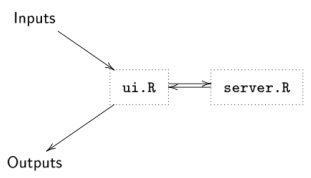
\includegraphics[width=7cm]{./Graficos/figura7}
\end{center}
\caption{Esquema interno de la aplicación.}
\label{fig:fig31}
\end{figure}


En las páginas y aplicaciones web se ha estandarizado el uso de ciertos lenguajes, tales como HTML, CSS, PHP o Javascript entre otros. Por defecto Shiny utiliza una plantilla básica de Twitter Bootstrap [18] para crear la interfaz de usuario, pero podemos descargar otras plantillas o crear una propia para personalizar nuestra aplicación. Twitter Bootstrap es un entorno de trabajo desarrollado por empleados de Twitter para fomentar la consistencia entre las herramientas internas, de forma que todas siguieran el mismo estilo. En 2011 Twitter liberó Bootstrap como código abierto, permitiendo que cualquiera lo usara para diseñar sus sitios o aplicaciones web. Contiene elementos de diseño basado en HTML, CSS y Javascript. Una de las mayores ventajas de Bootstrap es que permite crear interfaces web con CSS y JavaScript que adaptan la interfaz dependiendo del tamaño del dispositivo en el que se visualice de forma nativa, es decir, automáticamente se adapta al tamaño de un ordenador o de una tablet sin que el usuario tenga que hacer nada. Esto se denomina diseño adaptable o Responsive Design.

En lugar de usar un CSS propio para la interfaz de la aplicación se ha usado el paquete de R shinythemes [8], publicado por los creadores del propio Shiny. Shinytemes ofrece una serie de estilos básicos para aplicaciones Shiny.



\section{Creación de la Shiny APP}
%http://www.rpubs.com/JohanMarin/Shiny
La instalación de este paquete puede realizarse a través de los menús de Rstudio o simplemente con la siguiente orden:\\

\begin{lstlisting}[frame=single]
install.packages(shiny)
\end{lstlisting}

Para crear una Shiny app en \emph{File} se elige la opción Shiny Web App (figura \ref{fig:fig32}).

\begin{figure}[h]
\begin{center}
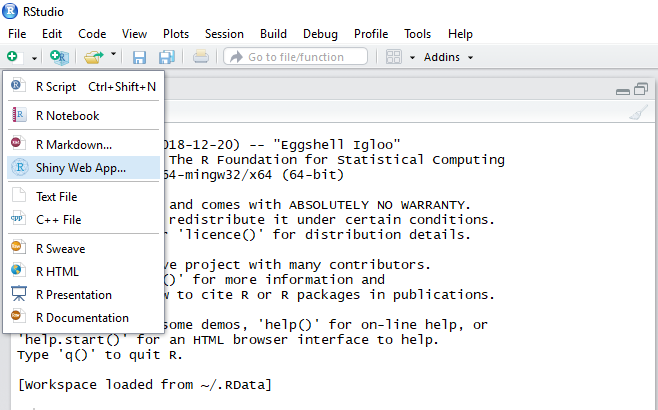
\includegraphics[width=12cm]{./Graficos/figura4}
\end{center}
\caption{Creación de Shiny Web App desde Rstudio}
\label{fig:fig32}
\end{figure}


Las aplicaciones Shiny están compuestas por un archivo app.R o dos archivos ui.R y server.R, es decir, se puede partir de un solo fichero que aglutine todo el código o se puede partir de dos archivos que separan la parte cliente de la parte servidora.

En este trabajo, se crea la aplicación Shiny mediante un unico script llamado app.R. El mismo se encuentra en un directorio (por ejemplo newdir/) y la aplicación se puede ejecutar con runApp(``newdir''). El script app.R esta formado por tres componentes:

\begin{itemize}
\item ui (\emph{user interfaz}): la interfaz de usuario controla el diseño de la aplicación, recibe los inputs y
muestra los outputs en el navegador.
\item server, funciones de R que contienen las instrucciones que se necesitan para construir los resultados de los análisis incluidos en la aplicación.
\item shinyApp, función que crea objetos de aplicación Shiny a partir de ui / servidor.
\end{itemize}


El archivo app.R deberá comenzar cargando el paquete Shiny y finalizar con una llamada a shinyApp:\\

\begin{lstlisting}[frame=single]
library(shiny)
ui<- ...
server<- ...
shinyApp(ui = ui, server = server)
\end{lstlisting}

La sesión de R estará monitoreando la aplicación y ejecutando las reacciones de la aplicación mientras la aplicación Shiny esté activa, por lo que no podrá ejecutar ningún comando.

La Figura \ref{fig:fig33} muestra el diseño utilizado en la aplicación. Se cuenta con un titulo y diferentes pestañas que conducen a diferentes páginas de la aplicación (\textbf{A}). Se cuenta con un panel de barra lateral (\textbf{B}), que contiene principalmente widgets con los cuales el usuario puede determinar el análisis que desea realizar y un panel principal (\textbf{C}) en el cual se obtenene los resultados del análisis solicitado.

\begin{figure}[h]
\begin{center}
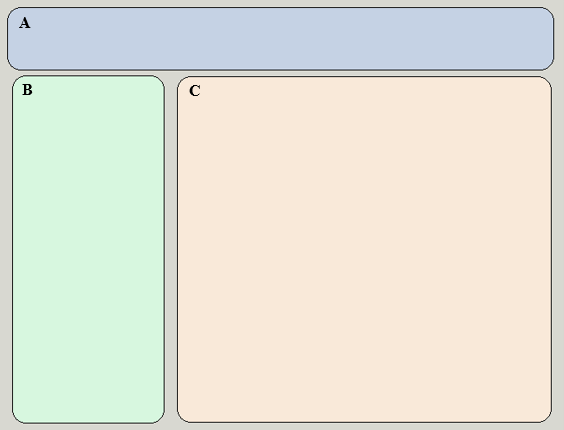
\includegraphics[width=12cm]{./Graficos/figura6}
\end{center}
\caption{Diseño de la aplicación Shiny. \textbf{A}: título y pestañas; \textbf{B}: área de entrada; \textbf{C}: área de resultados.}
\label{fig:fig33}
\end{figure}

\subsection{Tipos de componentes de Shiny Web App}

Los tipos de componentes de una aplación Shiny son:
\begin{itemize}
\item Componentes de Inputs y Outputs. Entre los inputs se encuentran numericInput, sliderInput, textInput, checkboxInput, entre otros. Posibles outputs se encuentran en la tabla \ref{tab:tabla1}, con las correspondientes funciones para server.R y ui.R
\item Componentes de Diseño. Algunos ejemplos se muestra en la tabla \ref{tab:tabla2}.
\item Componentes HTML (tags).
\end{itemize}


\begin{table}[h]
\begin{center}
\caption{Funciones para Outputs tanto para server.R como para ui.R}
\label{tab:tabla1}
\resizebox{\textwidth}{!} {
\begin{tabular}{cccc}
\hline
server.R & ui.R & espera & crea \\
\hline 
renderPlot & plotOutput & Gráfica & Gráfica\\
renderPrint & verbatimTextOutput, htmlOutput& salida impresa & texto\\
renderTable & tableOutput & objetos como tablas & tabla simple\\
renderDataTable & dataTableOutput & objetos como tablas & tabla DataTables.js\\
downloadHandler	& downloadButton, downloadLink & &\\
\hline 
\end{tabular}
}
\end{center}
\end{table}

\subsubsection{Componentes de Diseño}
% http://rstudio-pubs-static.s3.amazonaws.com/21373_8af3d3634b97461089c8a76659982915.html#componentes-shiny
\begin{itemize}
\item navbarPage(): Crea una página con una barra de navegación de nivel superior.
\item tabPanel(): Crea un panel de pestañas.
\item sidebarLayout(): Diseña de una barra lateral y el área principal.
\item sidebarPanel(): Crea un panel de barra lateral.
\item mainPanel(): Crea un panel principal.
\item navlistPanel(): Crea un panel de lista de navegación.
\item prettyRadioButtons(): Crea botones que permiten seleccionar un elemento de una lista.
\item materialSwitch(): Crea un interruptor de palanca para activar o desactivar una selección.
\item pickerInput(): Crea un control de selección de entrada.
\item navbarMenu():
\end{itemize}

{\small
\begin{table}[h]
\begin{center}
\caption{Componentes de Diseño de Shiny Web App}
\label{tab:tabla2}
\resizebox{0.6\textwidth}{!} {
\begin{tabular}{cccc}
\hline 
Componente	& Subcomponente	 \\
\hline
navbarPage(): & tabPanel(), navbarMenu()\\
navbarMenu() & tabPanel() \\
navlistPanel() & tabPanel()\\
titlePanel() &	\\
sidebarLayout() & sidebarPanel()  mainPanel() (obligatorio)	\\
sidebarPanel() & \\
mainPanel() & \\
tabsetPanel() &	\\
tabPanel()	 & \\
\hline
\end{tabular}
}
\end{center}
\end{table}
}


Para más información sobre estas componentes ver hoja de referencia de Shiny (Apéndice A).


\subsection{Compartiendo una Shiny Web App}

Una vez creada la aplicación, resulta conveniente ponerlas a disposición de los usuarios. En este caso la Shiny Web App encuentra disponible en el servidor de CONICET \url{www.cefobi.com}. Además el proyecto se encuentra en GitHub \url{https://github.com/jangelini/shinyAPP_geneticae}. 
